\section{Results}
\subsection{Localization precision of the microscope}
100 images acquired for every wavelength.
Then choosing a single molecule, \software{Scipy} library was used for two-dimensional gaussian fit.

\begin{figure}[htbp]
    \centering
    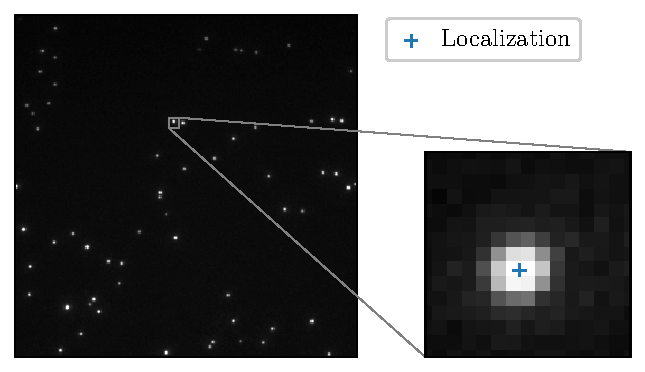
\includegraphics[scale=1]{figures/beads_inset_zoom.pdf}
    \label{fig:beads_inset_zoom}
    \caption{Whole acquisition and zoom on fluorescent beads which was studied. MUST FIX: la fenetre (les lims) n'est pas la même.}
\end{figure}


\subsection{STORM imaging of micro-tubules}
\begin{figure}[htbp]
    \begin{subfigure}{0.5\textwidth}    % trim left bottom right top
        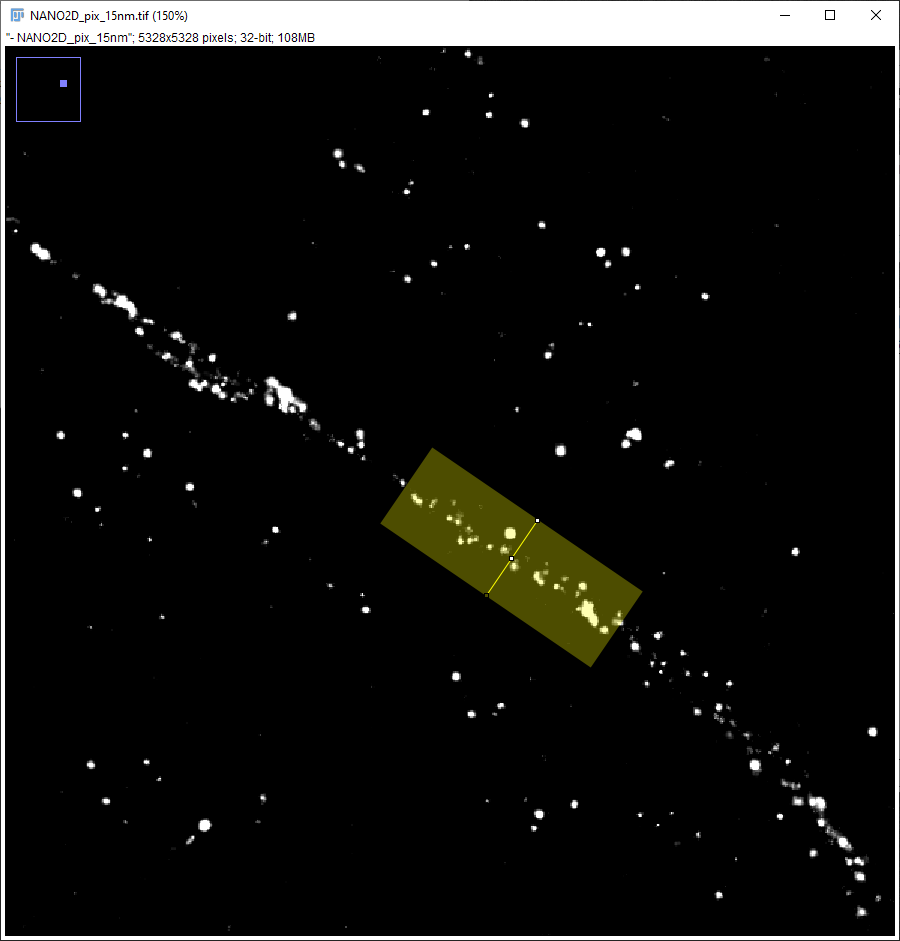
\includegraphics[width=\textwidth, trim={1cm 1.5cm 1cm 5cm}, clip]{figures/microtubules_width_acquisition.PNG}
        \caption{}
        \label{fig:microtubules_width_acquisition}
    \end{subfigure}
    \begin{subfigure}{0.5\textwidth}
        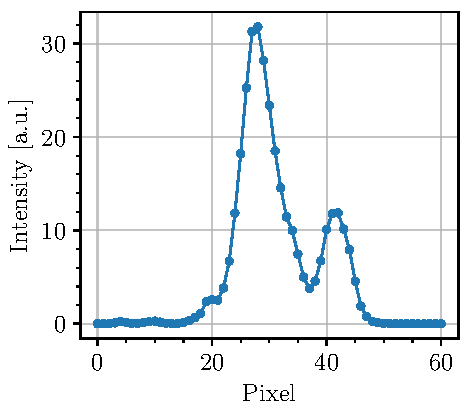
\includegraphics[scale=1]{figures/microtubules_width.pdf}
        \caption{}
        \label{fig:microtubules_width_analysis}
    \end{subfigure}
    \label{fig:microtubules_width}
    \caption{Intensity profile along a microtubule strand?}
\end{figure}

\begin{figure}
    \begin{subfigure}{0.32\textwidth}
        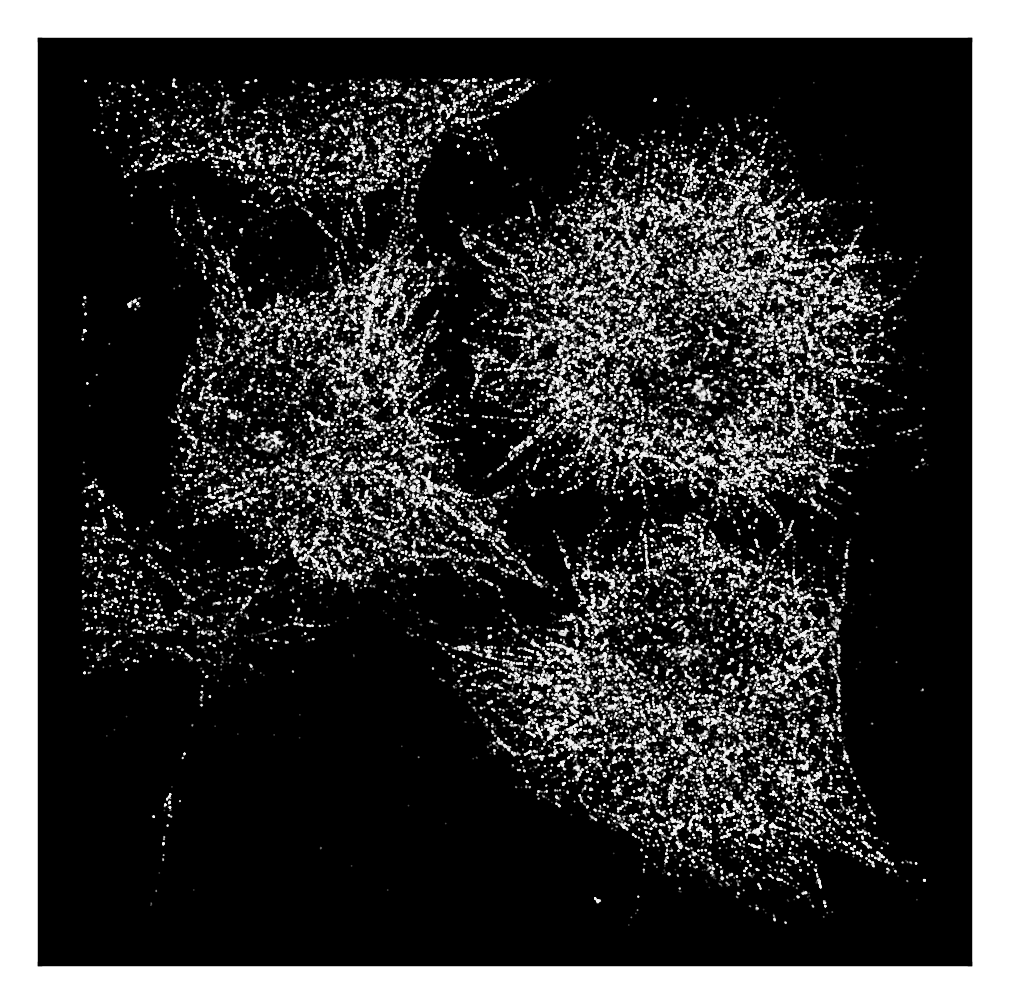
\includegraphics[width=\textwidth]{figures/test_scatter.png}
        \caption{}
    \end{subfigure}
    \begin{subfigure}{0.32\textwidth}
        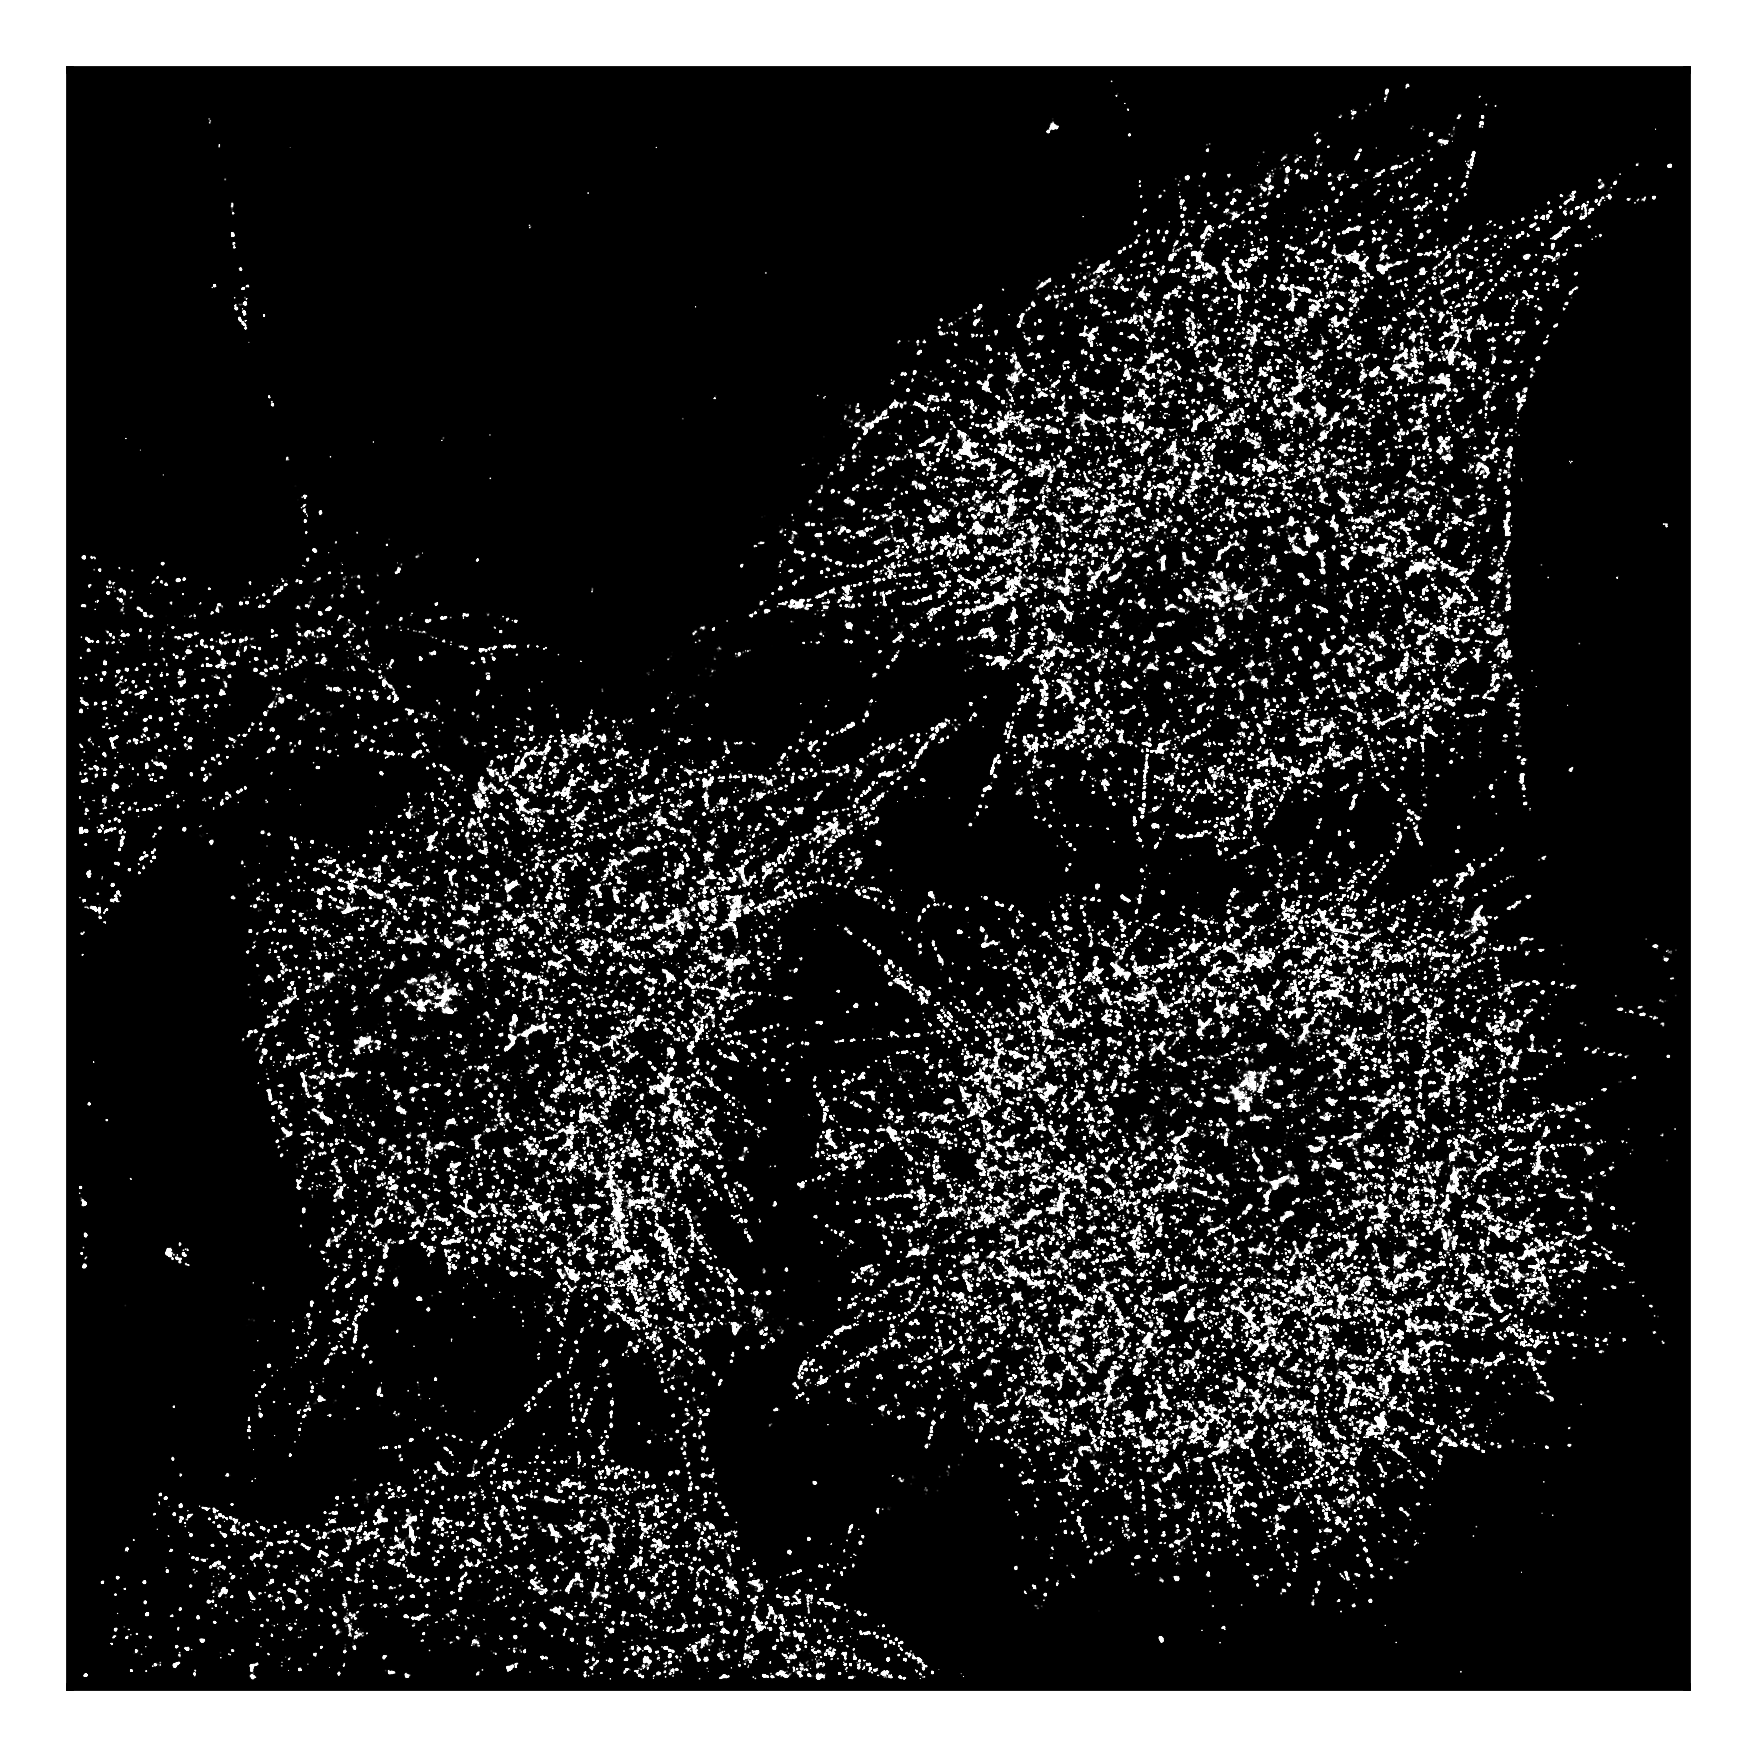
\includegraphics[width=\textwidth]{figures/test_imshow.png}
        \caption{}
    \end{subfigure}
    \begin{subfigure}{0.32\textwidth}
        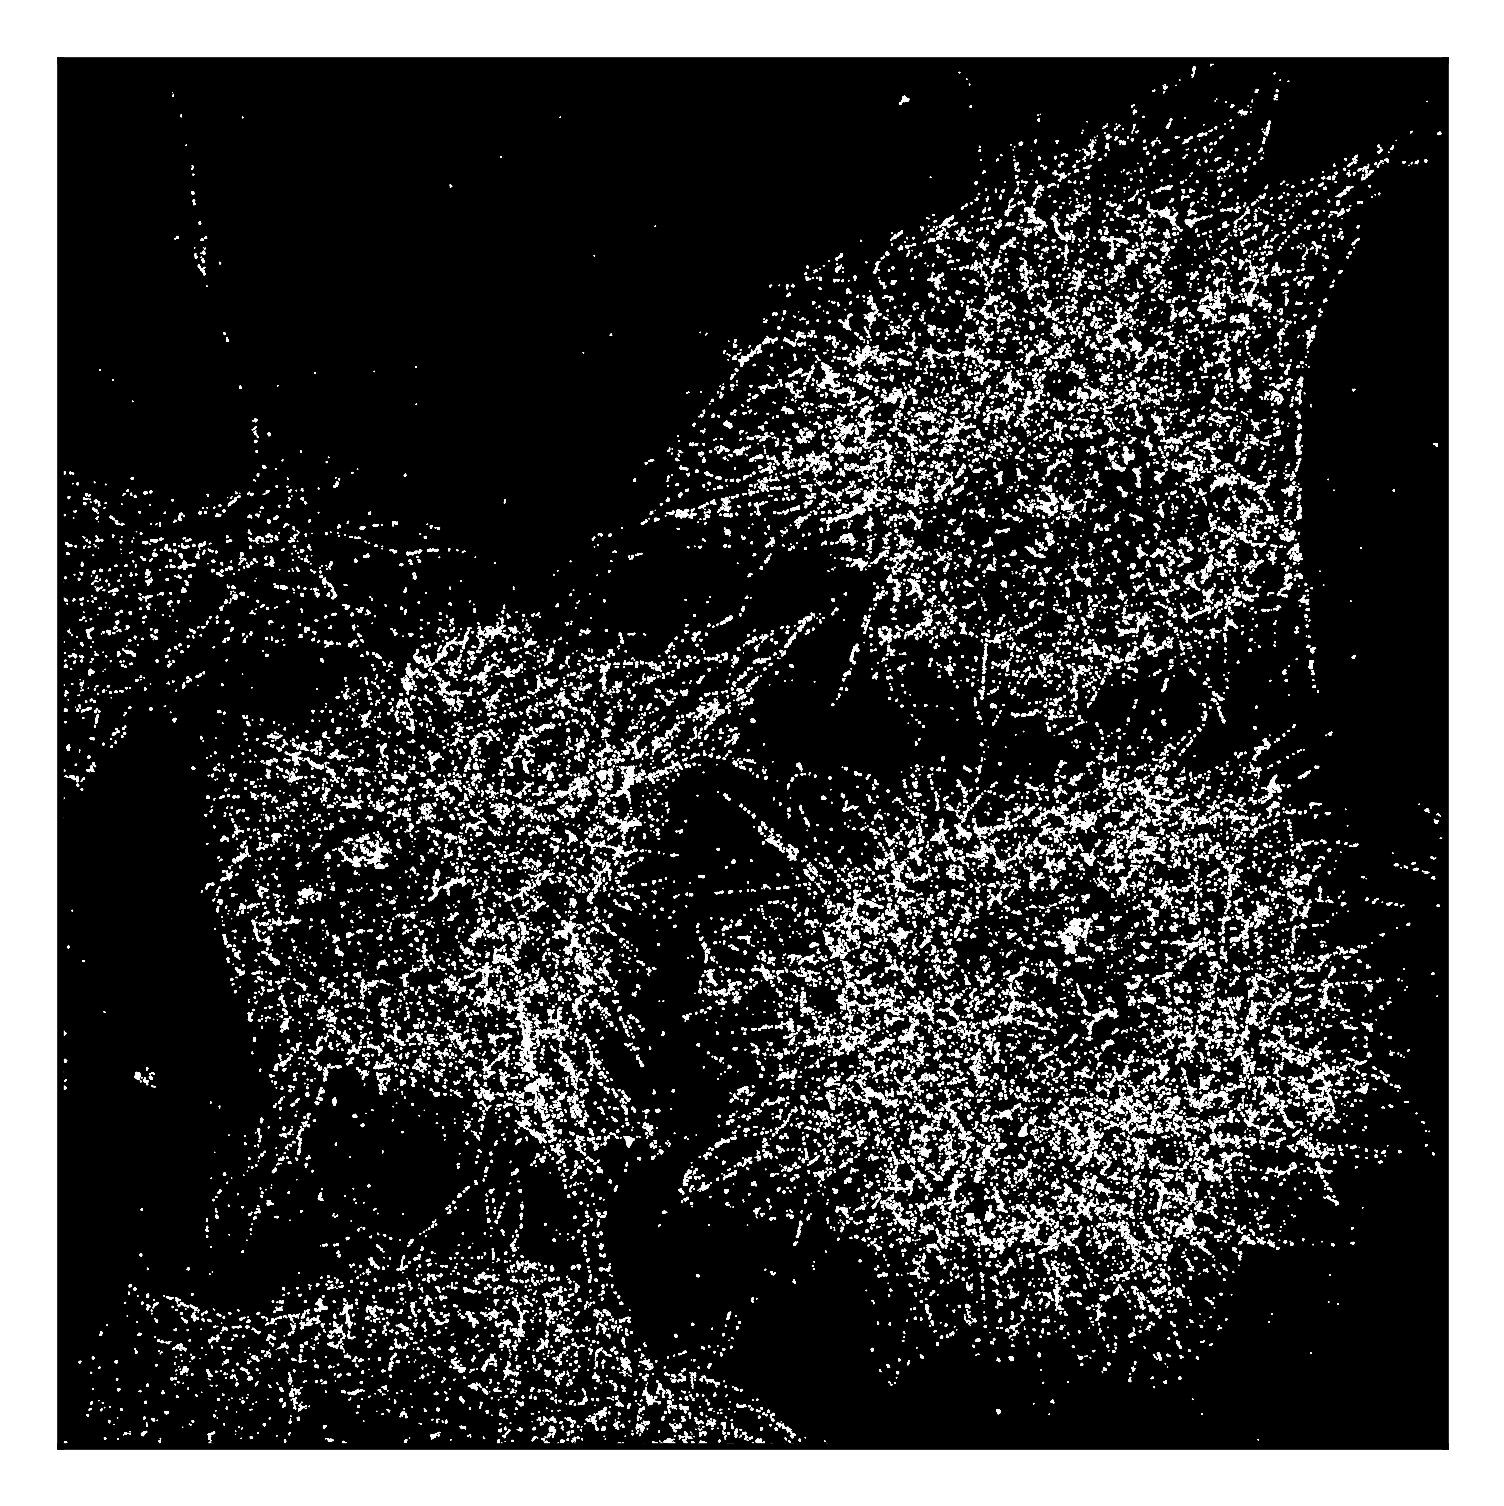
\includegraphics[width=\textwidth]{figures/gaussian_test.png}
        \caption{}
    \end{subfigure}
    \caption{Comparaison des différentes manières de former une image
    (a) scatter, (b) tiff, (c) gaussian magic}
\end{figure}